\documentclass[tikz,border=10pt]{standalone}
\usetikzlibrary{shapes.geometric, arrows.meta, positioning, calc, fit, backgrounds}

% Professional ACM/IEEE Academic Blue Palette
\definecolor{ieeePrimary}{RGB}{15, 65, 120}       % Deep Navy Blue
\definecolor{ieeeSecondary}{RGB}{40, 110, 170}   % Steel Blue
\definecolor{ieeeAccent}{RGB}{65, 150, 210}      % Sky Accent Blue
\definecolor{ieeeDarkGray}{RGB}{45, 55, 70}       % Slate Text Gray
\definecolor{ieeeLightBg}{RGB}{245, 248, 252}    % Node Shading Gray
\definecolor{ieeeBoxBg}{RGB}{255, 255, 255}      % Card White Fill
\definecolor{ieeeGroupBg}{RGB}{236, 242, 249}    % Layer Grouping Fill

\begin{document}
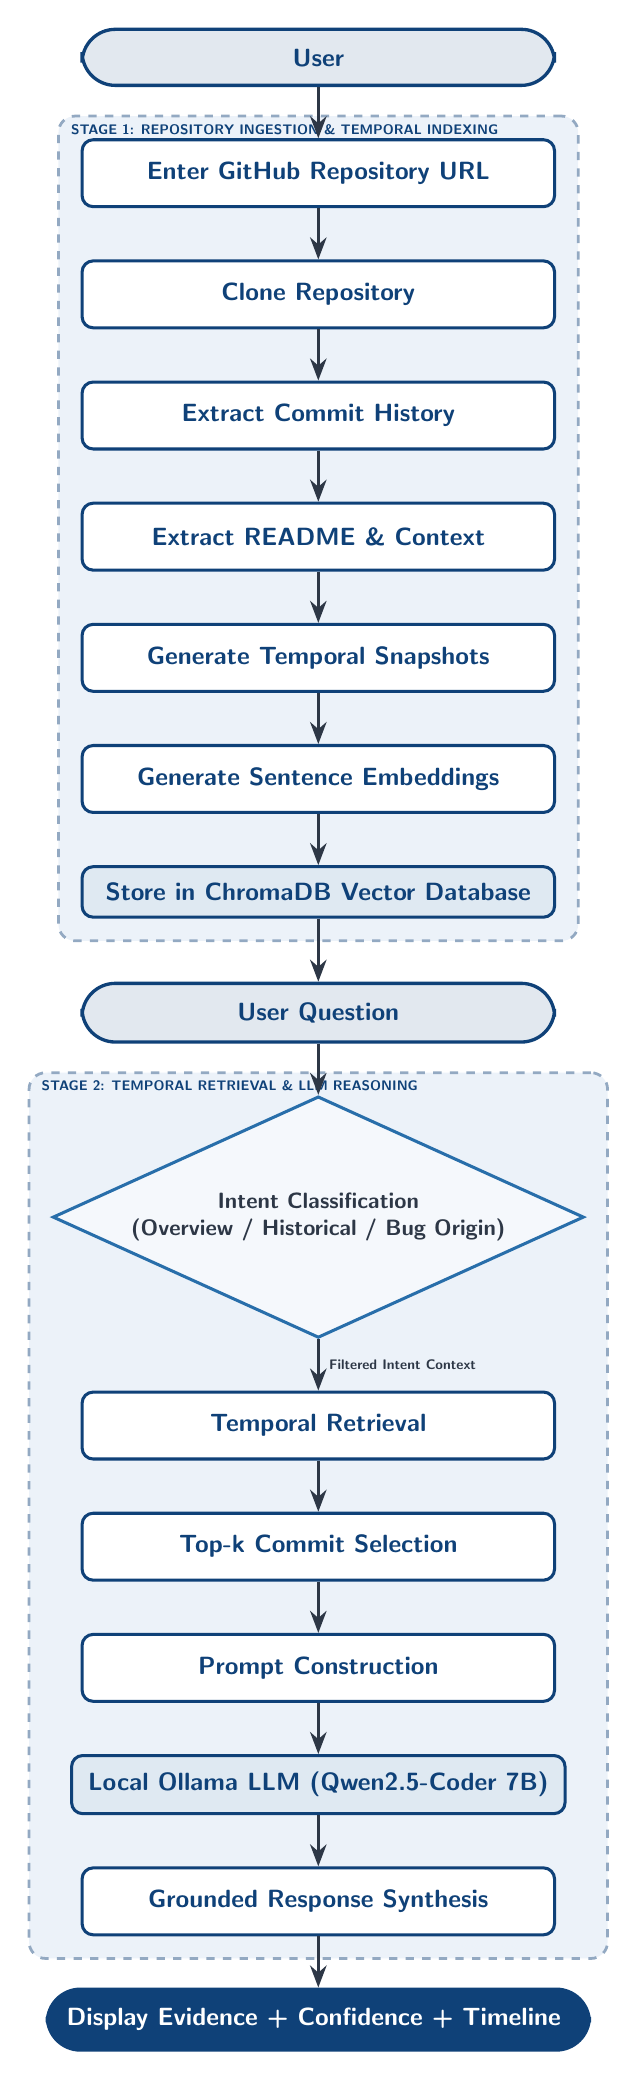
\begin{tikzpicture}[
    font=\sffamily\small,
    >=Stealth,
    node distance=0.65cm and 1.2cm,
    % Standard Process Block
    process/.style={
        draw=ieeePrimary,
        fill=ieeeBoxBg,
        rectangle,
        rounded corners=4pt,
        line width=1.1pt,
        align=center,
        inner sep=6pt,
        minimum width=6.0cm,
        minimum height=0.85cm,
        font=\sffamily\small\bfseries\color{ieeePrimary}
    },
    % Input / Terminal Node
    terminal/.style={
        draw=ieeePrimary,
        fill=ieeePrimary!12,
        rectangle,
        rounded corners=12pt,
        line width=1.2pt,
        align=center,
        inner sep=7pt,
        minimum width=6.0cm,
        font=\sffamily\small\bfseries\color{ieeePrimary}
    },
    % Decision Diamond Style
    decision/.style={
        draw=ieeeSecondary,
        fill=ieeeLightBg,
        diamond,
        aspect=2.2,
        line width=1.1pt,
        align=center,
        inner sep=3pt,
        font=\sffamily\footnotesize\bfseries\color{ieeeDarkGray}
    },
    % Data Storage Node
    storage/.style={
        draw=ieeePrimary,
        fill=ieeeSecondary!15,
        rectangle,
        rounded corners=4pt,
        line width=1.1pt,
        align=center,
        inner sep=6pt,
        minimum width=6.0cm,
        font=\sffamily\small\bfseries\color{ieeePrimary}
    },
    % Container Layer Style
    container/.style={
        draw=ieeePrimary!45,
        fill=ieeeGroupBg,
        rectangle,
        dashed,
        rounded corners=6pt,
        line width=1.0pt,
        inner sep=8pt
    },
    % Arrow Connection Style
    arrow/.style={
        draw=ieeeDarkGray,
        ->,
        line width=1.1pt
    }
]

    % Stage 1: User & Repository Ingestion Phase
    \node (user) [terminal] {User};
    \node (url) [process, below=of user] {Enter GitHub Repository URL};
    \node (clone) [process, below=of url] {Clone Repository};
    \node (commits) [process, below=of clone] {Extract Commit History};
    \node (readme) [process, below=of commits] {Extract README \& Context};
    \node (snapshots) [process, below=of readme] {Generate Temporal Snapshots};
    \node (embeddings) [process, below=of snapshots] {Generate Sentence Embeddings};
    \node (chromadb) [storage, below=of embeddings] {Store in ChromaDB Vector Database};

    % Stage 2: Conversational Retrieval & Reasoning Phase
    \node (question) [terminal, below=0.8cm of chromadb] {User Question};
    \node (intent) [decision, below=of question] {Intent Classification\\(Overview / Historical / Bug Origin)};
    \node (retrieval) [process, below=of intent] {Temporal Retrieval};
    \node (topk) [process, below=of retrieval] {Top-k Commit Selection};
    \node (prompt) [process, below=of topk] {Prompt Construction};
    \node (llm) [storage, below=of prompt] {Local Ollama LLM (Qwen2.5-Coder 7B)};
    \node (response) [process, below=of llm] {Grounded Response Synthesis};
    \node (display) [terminal, fill=ieeePrimary, text=white, below=of response] {
        Display Evidence + Confidence + Timeline
    };

    % Layer Grouping Containers
    \begin{scope}[on background layer]
        \node (ingest_layer) [container, fit=(url) (clone) (commits) (readme) (snapshots) (embeddings) (chromadb)] {};
        \node[anchor=north west, font=\sffamily\tiny\bfseries\color{ieeePrimary}] at (ingest_layer.north west) {\;STAGE 1: REPOSITORY INGESTION \& TEMPORAL INDEXING};

        \node (rag_layer) [container, fit=(intent) (retrieval) (topk) (prompt) (llm) (response)] {};
        \node[anchor=north west, font=\sffamily\tiny\bfseries\color{ieeePrimary}] at (rag_layer.north west) {\;STAGE 2: TEMPORAL RETRIEVAL \& LLM REASONING};
    \end{scope}

    % Connector Arrows
    \draw [arrow] (user) -- (url);
    \draw [arrow] (url) -- (clone);
    \draw [arrow] (clone) -- (commits);
    \draw [arrow] (commits) -- (readme);
    \draw [arrow] (readme) -- (snapshots);
    \draw [arrow] (snapshots) -- (embeddings);
    \draw [arrow] (embeddings) -- (chromadb);
    
    \draw [arrow] (chromadb) -- (question);
    \draw [arrow] (question) -- (intent);
    \draw [arrow] (intent) -- node[right, font=\sffamily\tiny\bfseries, color=ieeeDarkGray] {Filtered Intent Context} (retrieval);
    \draw [arrow] (retrieval) -- (topk);
    \draw [arrow] (topk) -- (prompt);
    \draw [arrow] (prompt) -- (llm);
    \draw [arrow] (llm) -- (response);
    \draw [arrow] (response) -- (display);

\end{tikzpicture}
\end{document}
